\documentclass[a4paper, 11pt]{article}
\usepackage{geometry}
\usepackage{graphicx}
\usepackage{a4wide}
\usepackage{ulem}
\usepackage{amsthm}
\usepackage{amsmath}
\usepackage{amsfonts}
\usepackage{amssymb}
\usepackage[T1]{fontenc}
\usepackage{ngerman}
\usepackage{graphicx}
\usepackage{epic}
\usepackage{enumerate}
\usepackage{tabu}
\usepackage [latin1]{inputenc}
\usepackage{algorithmic}
\usepackage{algorithm}
\geometry{a4paper,left=15mm,right=25mm,top=20mm,bottom=25mm}
%\renewcommand{\baselinestretch}{1.5}
\newcommand{\ol}{\overline}
\newcommand{\makeline}{\hrule\vspace{5pt}}
\newcommand{\ip}[2]{\left< #1, #2 \right>}

\title{11. �bungsblatt zu Software Qualit�t}
\author{Michel Meyer, Manuel Schwarz}

\begin{document}
  \maketitle

  \section*{Aufgabe 11.1 - Mutationen-Test}
  \subsection*{(a) Mutanten}
  Siehe *.java-Dateien \texttt{Pow2M1 - Pow2M6}.

  \subsection*{(b) Starker Mutationstest}
  Die Tabelle~\ref{tab:strong_mutation} zeigt die Ergebnisse des starken Mutationstests.
  Dabei steht eine \texttt{1} f�r einen erkannten Mutanten und eine \texttt{0} f�r einen
  nicht erkannten Mutanten.
  \begin{table}[htb!]
  \centering
  \caption{Ergebnisse des starken Mutationstests.}
  \label{tab:strong_mutation}
  \begin{tabular}[c]{|l|c|c|c|c|c|c|}\hline
             & M1 & M2 & M3 & M4 & M5 & M6 \\\hline\hline
  Testfall A & 0  & 1  & 1  & 1  & 0  & 0  \\\hline
  Testfall B & 0  & 1  & 1  & 1  & 0  & 1  \\\hline
  Testfall C & 0  & 1  & 0  & 0  & 0  & 0  \\\hline
  \end{tabular}
  \end{table}
  Der \textit{Test B} ist der beste, da dieser 4/6 Mutanten erkennt. \textit{Test C} hingegen erkennt nur
  1/6 Mutanten und ist damit der schlechteste.

  \subsection*{(c) Score}
  F�r den Score gilt folgende Formel:
  \begin{equation}
    Score = \frac{\text{Anzahl erkannter Mutanten}}{\text{Anzahl aller Mutanten - Anzahl �quivalenter Mutanten}}
  \end{equation}
  Dabei ist ein Mutant zum Original �quivalent, wenn keine Testf�lle existieren, die den Mutanten
  als solchen identifizieren k�nnen. Ist der Score eines Testfalles \texttt{1}, so nennt man diesen
  \textit{ad�quat}.
  \begin{align*}
    \text{Test A:}\,\,\,Score &= \frac{3}{6 - 2} = 0.75\\
    \text{Test B:}\,\,\,Score &= \frac{4}{6 - 2} = 1.0\\
    \text{Test C:}\,\,\,Score &= \frac{1}{6 - 2} = 0.25\\
  \end{align*}
  Damit ist \textit{B} ein \textit{ad�quater} Testfall.

  \subsection*{(d) Beispiel}
  Als Beispiele dienen die Klassen \texttt{Pow2.java} und \texttt{Pow2M1.java}, da diese �quivalent sind.
  In \texttt{Pow2M1.java} steht\\
  ------------------
  \begin{algorithmic}
    \STATE i = n
    \IF{(n $<$ 1)}
      \STATE i = -n
    \ENDIF
  \end{algorithmic}
  ------------------\\
  Dies ist �quivalent zu:\\
  ------------------
  \begin{algorithmic}
    \STATE i = n
    \IF{(n $<$ 0)}
      \STATE i = -n
    \ENDIF
    \IF{(n == 0)}
      \STATE i = -n
    \ENDIF
  \end{algorithmic}
  ------------------\\
  Und da $-0 = 0$ sind \texttt{Pow2.java} und \texttt{Pow2M1.java} �quivalent.\\\\
  Ein weiteres Beispiel k�nnte ein Programm mit der Zeile\\
  ------------------
  \begin{algorithmic}
    \IF{(a == b)}
      \STATE do stuff
    \ENDIF
  \end{algorithmic}
  ------------------\\
  sein. Durch eine erste Mutation k�nnte dies dann so aussehen:\\
  ------------------
  \begin{algorithmic}
    \IF{(a\,!= b)}
      \STATE do stuff
    \ENDIF
  \end{algorithmic}
  ------------------\\
  Und eine zweite Mutation k�nnte das Folgende verursachen:\\
  ------------------
  \begin{algorithmic}
    \IF{!(a\,!= b)}
      \STATE do stuff
    \ENDIF
  \end{algorithmic}
  ------------------\\
  Damit w�re dieser Mutant �quivalent zum Original.


  \section*{Aufgabe 11.2 - Stilanalyse}

    \subsection*{5.1.4 End-Of-Line Comments}
    Diese Konvention tr�gt dazu bei, dass erfahrene Java Programmierer schneller erkennen k�nnen,
    um was f�r Kommentare es sich handelt. Dabei soll ``//'' suggerieren, dass es sich (h�chstwahrscheinlich)
    um auskommentierten Code handelt und soll sich damit zu beispielsweise ``/* \dots */'' abgrenzen, da letzteres
    f�r tats�chliche, hilfreiche Kommentare genutzt wird. Ein Programmierer wei� dadurch sofort genau, wo er
    zu gucken hat, wenn er beispielsweise nach auskommentierten Code sucht.


    \subsection*{7.3 return Statements}
    A return statement with a value should not use parentheses unless they make the return value
    more obvious in some way. Example:\\\\
    \texttt{return;}\\\\
    \texttt{return myDisk.size();}\\\\
    \texttt{return (size\,? size : defaultSize);}\\\\
    Die Klammern wegfallen zu lassen ist aus zwei Gr�nden sinnvoll:
    \begin{itemize}
      \item Das statement ist als Satz lesbar: ``\texttt{return myDisk.size()}'' => ``gib \texttt{myDisk.size()} zur�ck''.
      \item Klammern (als Alternative) w�rden return als eine Funktion suggerieren, bei dem der R�ckgabewert
          als Parameter angegeben wird, was einer imperativen Sprache entgegen spr�che.
    \end{itemize}
    Daher gibt es auch Ausnahmef�lle wie oben, denn ``\texttt{return size\,? size : defaultSize;}'' w�rde sich vielmehr als
    ``\texttt{(return size)\,? size : defaultSize;}'' lesen, was nicht der Semantik (und Syntax) entspricht.

    \section*{Aufgabe 11.3 - Slicing}
    \subsection*{Kontrollflussgraph}
    \begin{figure}[htb!]
      \centering
      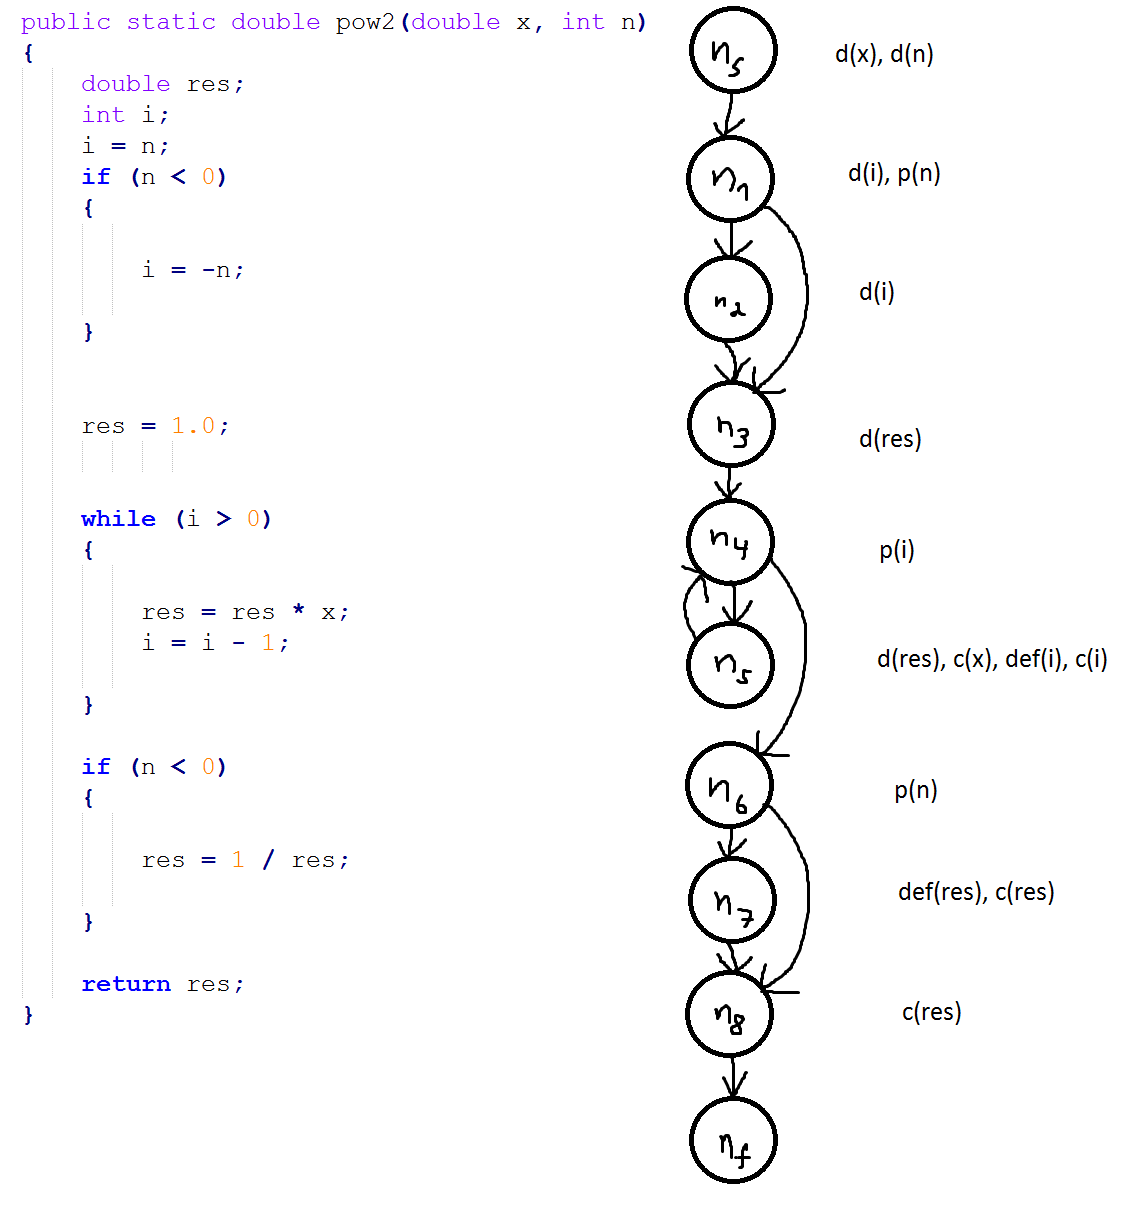
\includegraphics[width=0.8\textwidth]{Aufg3.png}
    \end{figure}


    \subsection*{(a) Forward und Backward-Slicing}
    \subsubsection*{\texttt{res}}
    \begin{figure}[htb!]
      \centering
      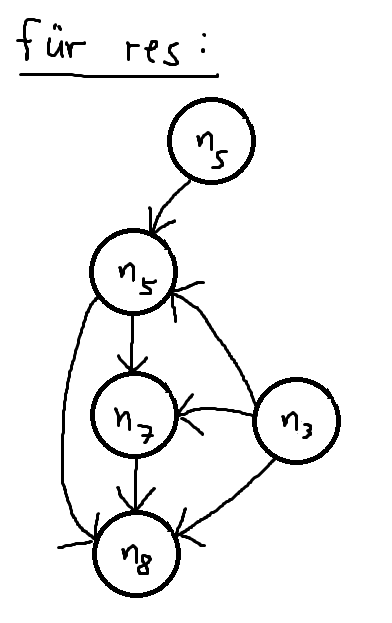
\includegraphics[width=0.25\textwidth]{Aufg3a_res.png}
    \end{figure}

    \subsubsection*{\texttt{i}}
    \begin{figure}[htb!]
      \centering
      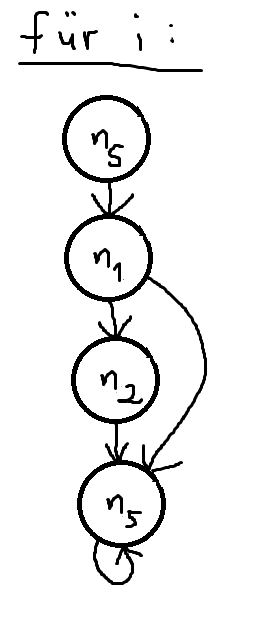
\includegraphics[width=0.25\textwidth]{Aufg3a_i.png}
    \end{figure}

    \subsection*{(b) Forward-Slicing f�r \texttt{i}}
    \begin{figure}[htb!]
      \centering
      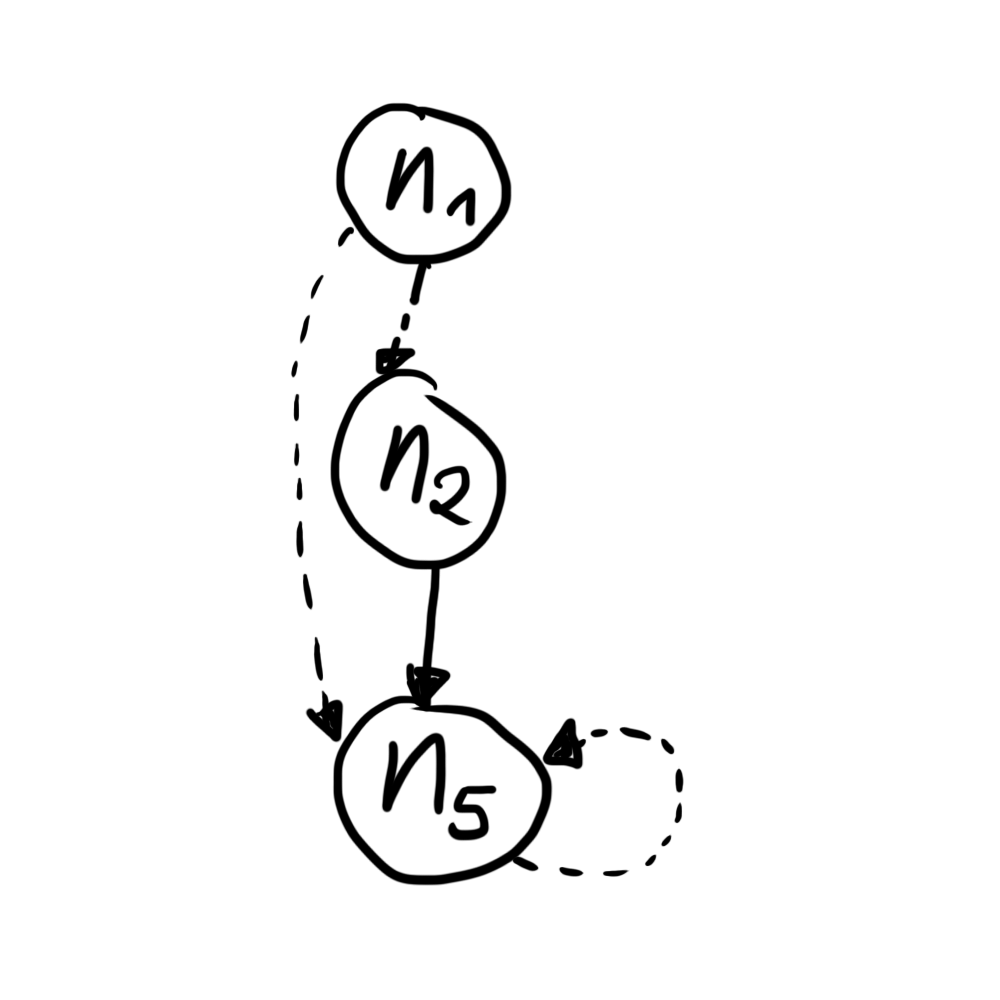
\includegraphics[width=0.15\textwidth]{Aufg3b.png}
    \end{figure}

\end{document}
